\chapter{Indledning incl. problemformulering}

\section{Baggrund}
En normal synkeproces er kendetegnet ved, at fødeindtagelsen, som passerer fra den bageste del af mundhulen via. svælget og spiserøret til mavesækken, sker uden besvær. Forstyrrelser i synkeprocessen, dens hastighed og frekvens kaldes for dysfagi \cite{Sundhedsstyrelsen2015NationalDysfagi}. Dysfagi er den medicinske betegnelse for symptom relateret til synkebesvær. Der er vigtigt at differentiere mellem nedre og øvre dysfagi. Øvre dysfagi omfatter den præ-orale, orale og faryngeale fase, hvorimod nedre dysfagi relaterer sig den øsefageale fase dvs. mavesæk og spiserør \cite{KjaersgaardPh.d.studerendeDYSFAGIKonsekvenser}. Det skal dog nævnes, at der er uenigheder om definitionen af dysfagi. Den manglende konsensus om definitionen gør rapportering af dysfagi insidens og prævalens uklar \cite{KjaersgaardPh.d.studerendeDYSFAGIKonsekvenser}. Ifølge patientombuddets temarapport fra 2012 om dysfagi at:

\begin{itemize}
\item 60-87 \% af beboere på plejehjem for ældre har synkebesværligheder.
\item 30 \% alle apopleksipatienter har dysfagi.
\item 20-50 \% af patienter med Parkinson og Alzheimer har dysfagi.
\item 30-60 \% af patienter med muskelsvind har dysfagi.
\item Herudover er der ca. 10.000 børn, unge og voksne med Cerebral Parese (CP) også kendt som "spastisk lammelse", der har synkebesvær \cite{Bommersholdt2012TemarapportDysfagi}. 
\end{itemize}

Som det ses i de nævnte statistikker, rammer dysfagi en bredt vifte af patienter fra forskellige patientgrupper. Dysfagi konsekvenserne kan læses i \nameref{bilag1}. 

Udredning af øvre dysfagi består af en diagnostisk strategi med tre trin: en tidlig screening, som skal afdække eksistensen af synkebesværligheder, en allround klinisk undersøgelse, der estimerer synkebesværlighedens omfang og en instrumentel undersøgelse vha. Fiber Endoskopisk Evaluering af Synkefunktionen (FEES) og/eller Funktionel Videoradiologisk Evaluering af Synkefunktionen (FVES). Alle nævnte undersøgelsesmetoder er manuelle undersøgelser, der indeholder flere subjektive vurderinger som klinikeren rapporterer undervejs i undersøgelsen og dette kan forringe undersøgelsens reproducerbarhed. Resultatet kan være underdiagnostik og derved dårlig tilrettelæggelse af et behandlingsforløb. I \nameref{bilag1} belyses hvordan FEES og FVES foretages. FEES og FVES anvendes til at dømme aspirationsrisiko og til at angive anbefalinger for oral indtagelse, men flere studier viser, at begge metoder ikke er tilstrækkelig pålidelige,  ofte ikke gentagelige og dyre i pris \cite{Kelly2006} \cite{McCullough2001Inter-Measures} \cite{Schultheiss2014} \cite{Nahrstaedt2012SwallowMeasurements}.  Der er derfor brug for alternative metoder, som kan give objektive detektioner af synke problemer. En af disse metoder er at kombinere elektromyografi (EMG) og bioimpedans sensorer. Et forudgående projekt til dette projekt har anvendt en prisvenlig EMG sensor af typen MyoWareTM Muscle Sensor til at måle synkesignaler på raske personer med succes \cite[s. 58]{ChristensenElisabethLundbakStrand2017}. Dette projekt anvender også den samme EMG sensor for at reproducere de samme resultater. EMG alene er ikke tiltrækkelig til at vurdere dysfagi, da den kun bidrager med informationer om muskelaktiviteten i de muskler, der deltager i synkningen \cite{Schultheiss2014}. Derfor anvender dette projekt en prisbillig bioimpedans sensor, som en gruppe forskere har anbefalet, samt beskrevet en opskrift til udviklingen af sådan en bioimpedans sensor \cite{Aroom2009}.

Bioimpedans er kompleks modstand, der kan anvendes til at måle den elektriske impedans i vævet ved at udnytte forholdet mellem spænding og strøm jf. Ohms lov. Ved væske- og/eller fødeindtagelse samt vejrtrækning ændres forholdet mellem spænding og strøm i svælget og det er denne ændring, som bioimpedans sensoren skal måle. Som det ses på figur \ref{EMGBIGraph}, er svælget åben og fuld af luft under vejtrækning. Luft er dårlig til at lede strøm og har en høj elektrisk modstand. Den høje elektriske modstand falder under synkning af væske eller mad ved at svælgets hulrum indsnævres, som et resultat af en opadgående bevægelse af hyoid og larynx. Dette observeres som et drop i bioimpedans signalet og lave svingninger i EMG signalet for raske personer. For personer med dysfagi vil droppet i bioimpedans signalet være lavere  \cite{Schultheiss2014}.  



\begin{figure}[H]
\centering
{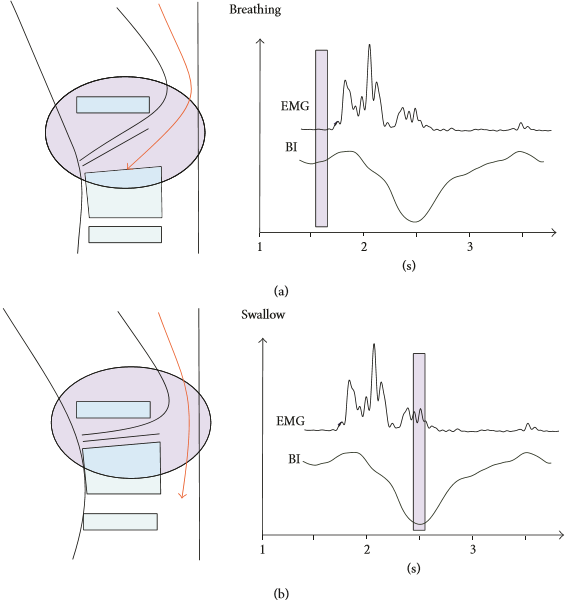
\includegraphics[width=9cm]
{Figure/EMGBIGraph}}
\caption{Viser, hvodan emg-og bioimpedans signaler opfører sig under vejrtrækning og mad/drikke indtagelse\cite{Schultheiss2014}}
\label{EMGBIGraph}
\end{figure}

\section{Problemformulering}

Dette projekt undersøger muligheden for at udvikle en bioimpedans sensor som kan monitorere og evaluere synkefrekvensen på raske personer. I projektoplægget til dette projekt er der henvist til en artikel\footnote{Bioimpedance Analysis: A Guide to Simple Design and Implementation}, som beskriver en opskrift til udvikling af en bioimpedans sensor. Projektet vil følge denne opskrift til udvikling af denne sensor. Projektet vil søge svar til følgende spørgsmål: 

\begin{itemize}
\item Er der evidens for en prisbillig bioimpedans sensor kan være alternativ til Fiber Endoskopisk Evaluering af Synkefunktionen (FEES) og Funktionel Videoradiologisk Evaluering af Synkefunktionen (FVES) til at undersøge synkefrekvensen på personer, der er ramt af dysfagi ?
\item Kan man kombinere bioimpedans sensor og EMG til måling af dysfagi ?

\end{itemize}
Ved hjælp af systematisk og ikke-systematisk litteratursøgning vil disse spørgsmål blive besvaret gennem dette projekt. 

\section{Formål}

Formålet med dette projekt er at udvikle et produkt, der består af en bioimpedans måler, der kan måle pålidelige bioimpedans signaler, samt kombinere bioimpedans måleren med en kommerciel EMG sensor for at kunne detektere synkefrekvensen på raske objekter, se figur \ref{KonceptuelDiagram}. Det overordnet systemet består af en bioimpedans måler med to elektroder som er koblet til et rask objekt, en EMG måler med tre elektroder, som også er koblet til det samme objekt og en pc som anvendes til processering og visning af data til et sundhedspersonale.  

\begin{figure}[H]
\centering
{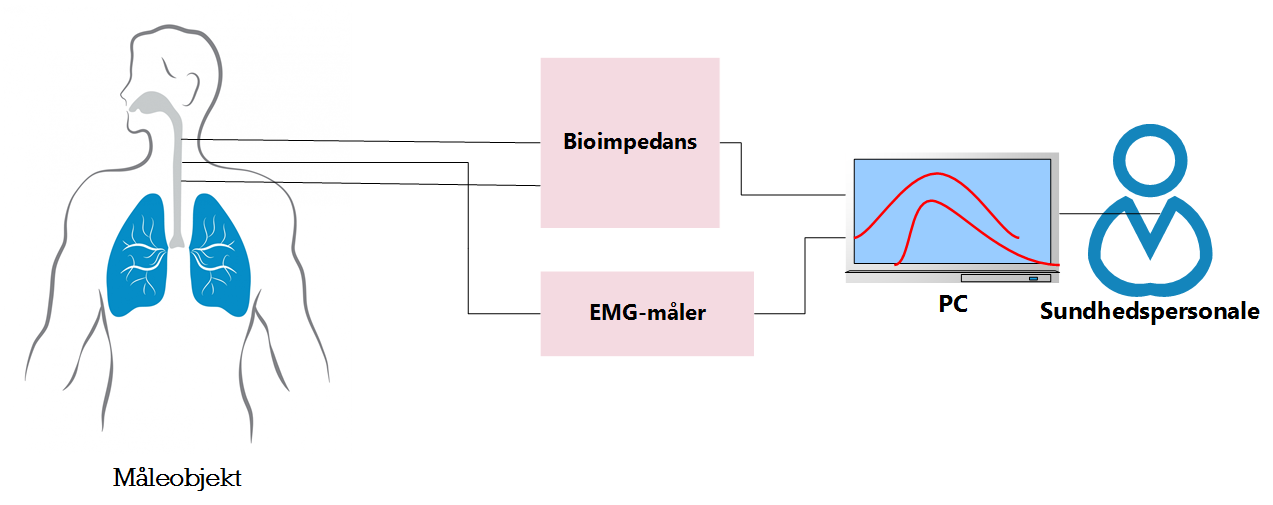
\includegraphics[width=11cm]
{Figure/KonceptuelDiagram}}
\caption{Viser det overordnet system som dette projekt vil realisere}
\label{KonceptuelDiagram}
\end{figure}

Projektet vil fokusere på udvikling af den udpegede prisbillige bioimpedans måler for at undersøge muligheden for at anvende bioimpedans måler til udredning af patienter med mistanke for dysfagi. Det er ligeledes projektets mål at genskabe de to signaler, der er vist i figur \ref{EMGBIGraph}. EMG måleren bruges som supplerende redskab til bioimpedans måleren, da den kan detektere muskelaktiviteter, som finder sted før, under og efter et synk. Disse muskelaktiviteter er en forudsætning for, at synkning kan ske. 

Det er ikke projektets mål at udvikle en endelig bioimpedans måler, der kan sættes i produktion eller anvendes til screening af personer med mistanke for dysfagi på kort sigt. Målet er at bygge en prototype af en bioimpedans måler, der først og fremmest kan måle synkefrekvens hos raske personer. 

\section{Samarbejdspartner}
Dette projekt gennemføres i samarbejde med Hammel Neurocenters Ambulatorium for Dysfagi og Endoskop, der ønsker at undersøge objektive alternative/supplerende metoder til at screene patienter med dysfagi. Fremover omtales Hammel Neurocenter som kunde til projektets produkt. 

%\section{Problemformulering}